%UNIT 7: MODELING WITH AUTONOMOUS DIFFERENTIAL EQUATIONS
%%%%%%%%%%%%%%%%%%%%%%%%%%%
%%%% Put the following at the top of each .tex file  %
\pagestyle{fancy}
\renewcommand{\theUnit}{7}
\ifthenelse{\isundefined{\UnitPageNumbers}}{}{\setcounter{page}{1}}
\rhead{Unit \theUnit: Modeling with Autonomous Differential Equations}
\lhead{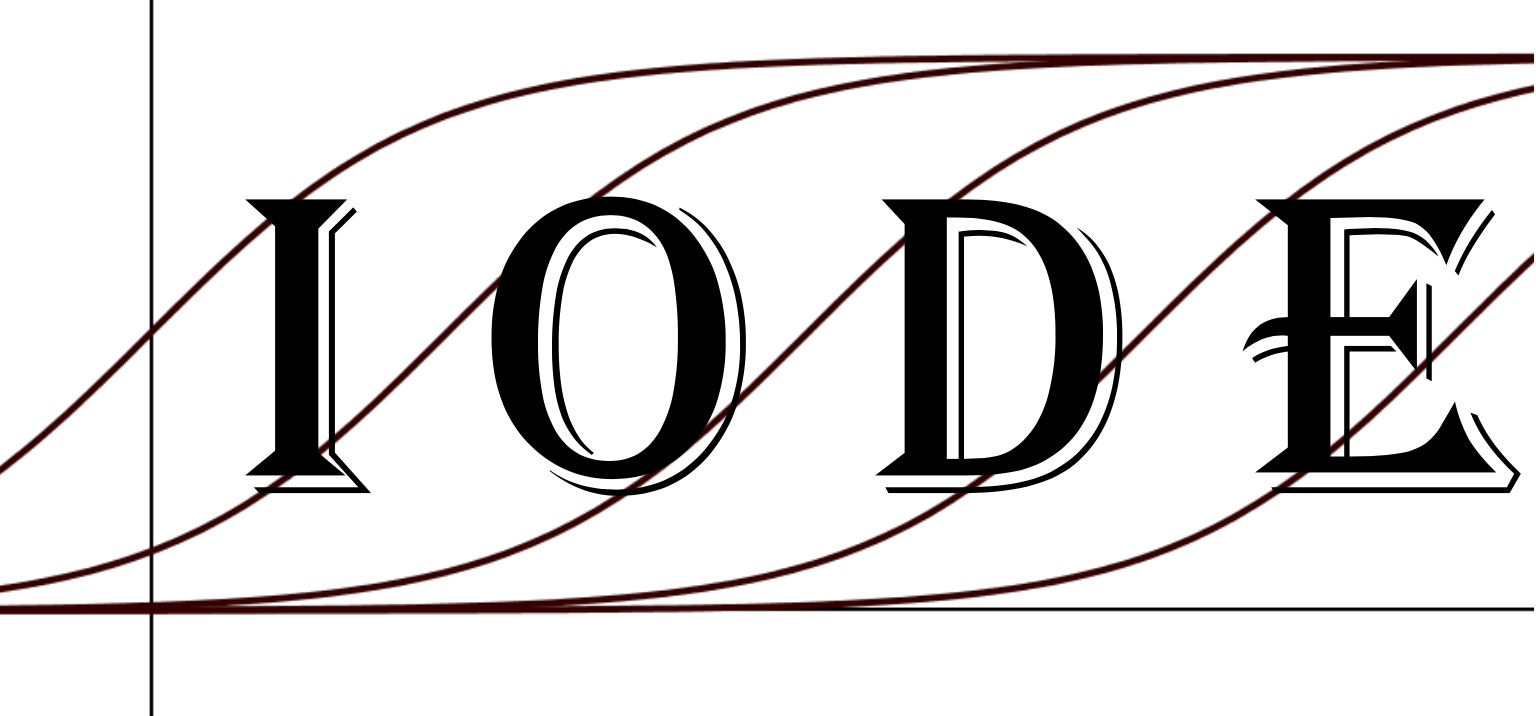
\includegraphics[width=1.25cm]{IODE-logo.png}}
\rfoot{\mypage}
\lfoot{}
\cfoot{}
\fancypagestyle{firstfooter}{\footskip = 50pt}
\renewcommand{\footrulewidth}{.4pt}
%%%%%%%%%%%%%%%%%%%%%%%%%%%
\vspace*{-20pt} \thispagestyle{firstfooter}
\pagebegin{Cooling Coffee}

\includegraphics[]{07/07CoffeeCup.png}
A group of students want to develop a rate of change equation to describe the cooling rate for hot coffee in order that they can make predictions about other cups of cooling coffee. Their idea is to use a temperature probe to collect data on the temperature of the coffee as it changes over time and then to use this data to develop a rate of change equation. \\

The data they collected is shown in the table below. The temperature C (in degrees Fahrenheit) was recorded every 2 minutes over a 14 minute period. \\

\begin{tabular}{|c|c|}
\hline
Time (min) & Temp. (\degree F)\\\hline
0 & 160.3\\\hline
2 & 120.4\\\hline
4 & 98.1\\\hline
6 & 84.8\\\hline
8 & 78.5\\\hline
10 & 74.4\\\hline
12 & 72.1\\\hline
14 & 71.5\\\hline
\end{tabular}
\begin{enumerate}
\item Figure out a way to use this data to create a third column whose values approximate  $\displaystyle\frac{dC}{dt}$, where $C$ is the temperature of the coffee.\label{07problem1} \vfill

\item	Do you expect $\displaystyle\frac{dC}{dt}$ to depend on just the temperature $C$, on just the time $t$, or both the temperature $C$ and the time $t$? \label{07problem2} \vfill

\item Sketch below your best guess for the graph of $\displaystyle\frac{dC}{dt}$. \label{07problem3}
\begin{center}
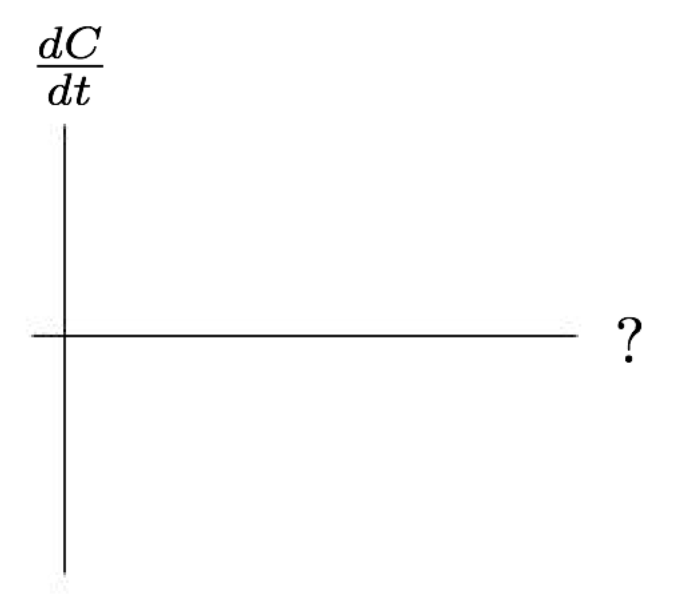
\includegraphics[width=3in]{07/07dCdt.png}
\end{center}

\clearpage
\item
\begin{enumerate} \label{07problem4} 
\item Input the data from your extended table in question \ref{07problem1} into the GeoGebra applet \\\href{https://ggbm.at/uj2gbz3V}{\underline{https://ggbm.at/uj2gbz3V}} to plot points for $\displaystyle\frac{dC}{dt}$ vs. $C$. Does this plot confirm or reject your sketch from question \ref{07problem3}? 
\vspace{1.5in}
\item Toggle on the curve fitting tool and find an equation that fits your data.
\end{enumerate} 

\vspace{-2in}\hspace{-0.5in}
\includegraphics[width=0.5in]{07/07CoolingCoffeeQR.png}
\vfill

\clearpage

\item One group of students figured out that a reasonable rate of change equation to be \[ \frac{dC}{dt}=-0.4C+28\]   which they rewrote as  \[\displaystyle \frac{dC}{dt}=-0.4\left(C-70\right).\] Interpret the meaning of the number $70$ in this equation. Does this rate of change equation also make sense for predicting the future temperature of a glass of ice tea? Why or why not? \label{07problem5}
\vfill
\item	According to the rate of change equation from questions \ref{07problem4} and \ref{07problem5}, is it possible for a graph of the \bf exact \rm solution to look like the one below? Why or why not? Give more than one reason for your answer. \label{07problem6}
\begin{center}
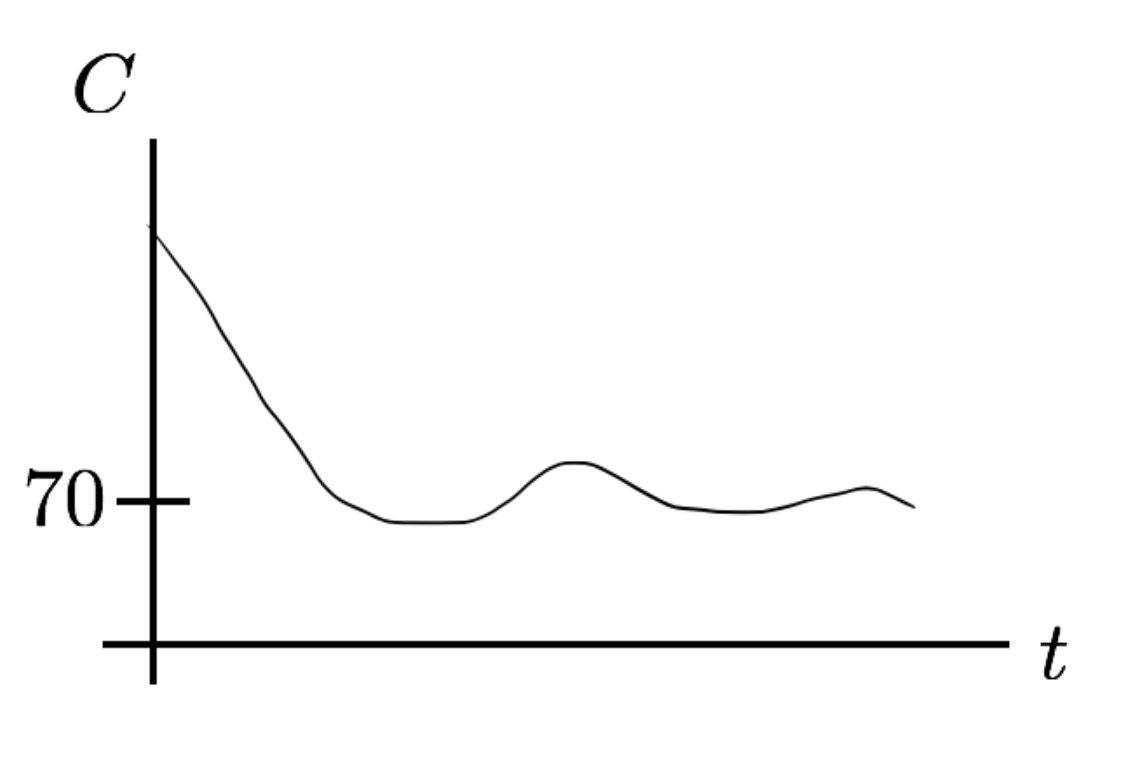
\includegraphics[width=3in]{07/07CoffeeEquilibrium.png}
\end{center}
\vfill

\end{enumerate}
\clearpage

%%%%%%%%%%%%%%%%%%%%%%%%%%%
\pagebegin{Population Growth - Limited Resources}
A group of biologists want to study the population growth of certain bacteria in a laboratory. The scientists realized that the culture for the bacteria does not provide unlimited resources. Hence, the rate of change equation $\displaystyle\frac{dP}{dt}=kP$ is not appropriate. They conducted experiments to determine how the rate of change of population depends on just the population. The data they collected is shown in the table below (numbers are properly scaled). At various population levels, the scientists measured the population after one day. \\

\begin{tabular}{|c|c|}
\hline
\parbox{1in}{Beginning\\ Population} & \parbox{1.5in}{Population after\\ one day}\\ \hline 
2 & 2.34\\ \hline 
4 & 4.54\\ \hline 
6 & 6.62\\ \hline 
8 & 8.58\\ \hline 
10 & 10.40\\ \hline 
12 & 12.10\\ \hline 
14 & 13.66\\ \hline 
16 & 15.10\\ \hline 
18 & 16.42\\ \hline 
20 & 17.60\\ \hline 

\end{tabular}

\begin{enumerate}[resume]
\item	Create a third column whose values approximate $\frac{dP}{dt}$. Explain why the method you used to create this column makes sense.\label{07problem7}\vfill



\item	In this course we will call a graph of $\frac{dP}{dt}$ vs. $P$, when $\frac{dP}{dt}$ is an autonomous differential equation, an \textbf{Autonomous Derivative Graph}. Create an \textbf{autonomous derivative graph} and figure out a way to analyze this graph to determine the long term behavior for each of the beginning populations given in the table above.\label{07problem8}
\vfill
\end{enumerate}

\clearpage

%%%%%%%%%%%%%%%%%%%%%%%%%%%%%%%
\pagebegin{Analyzing Graphs of Autonomous Differential Equations}

\begin{enumerate}[resume]
\item A group of biologists is studying a particular bug population in a rainforest. They gathered data about these bugs for different population values, $N$, at different times, $t$. The scientists reasoned that the rate of change depended only on the population and not on time. They approximated the derivatives $\frac{dN}{dt}$ (as was done with the cooling coffee from before) and plotted the autonomous derivative graph, as seen below: \label{07problem9}
\begin{center}
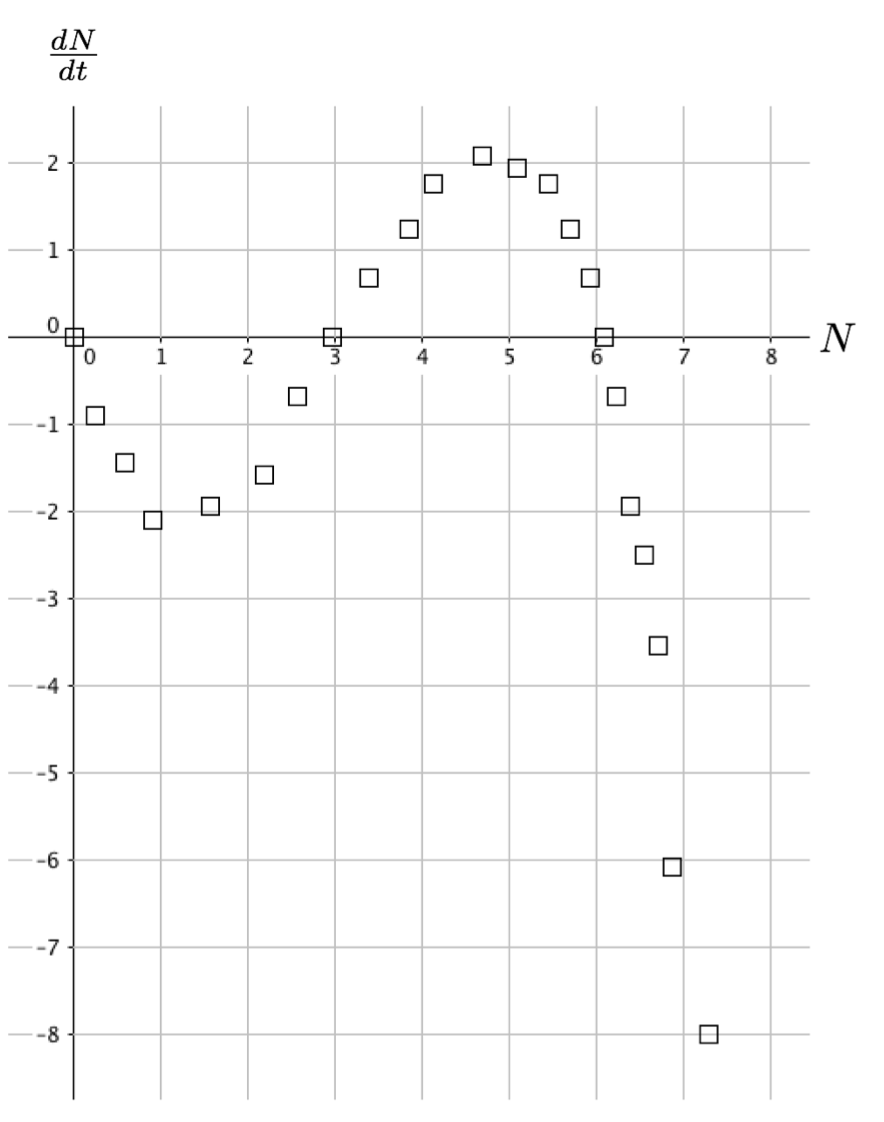
\includegraphics[width=3.5in]{07/07Bugs1.png}
\end{center}
For each part below, use the autonomous derivative graph to predict what the ultimate fate of the population will be. Describe (in words) the long-term behavior of each solution corresponding to the given initial condition. In addition, illustrate your conclusions with a suitable graph or graphs and classify all equilibrium solutions as either an attractor, repeller, or node.

\begin{enumerate}
\item	$N(0) = 2$ 
\item	$N(0) = 3$
\item	$N(0) = 4$
\item	$N(0) = 4.5$
\item	$N(0) = 6$
\item	$N(0) = 8$
\end{enumerate}

\clearpage
\item	Below is an autonomous derivative graph. Figure out the long-term behavior of \underline{every} possible solution function and illustrate your conclusions with a suitable graph or graphs. \label{07problem10}
\begin{center}
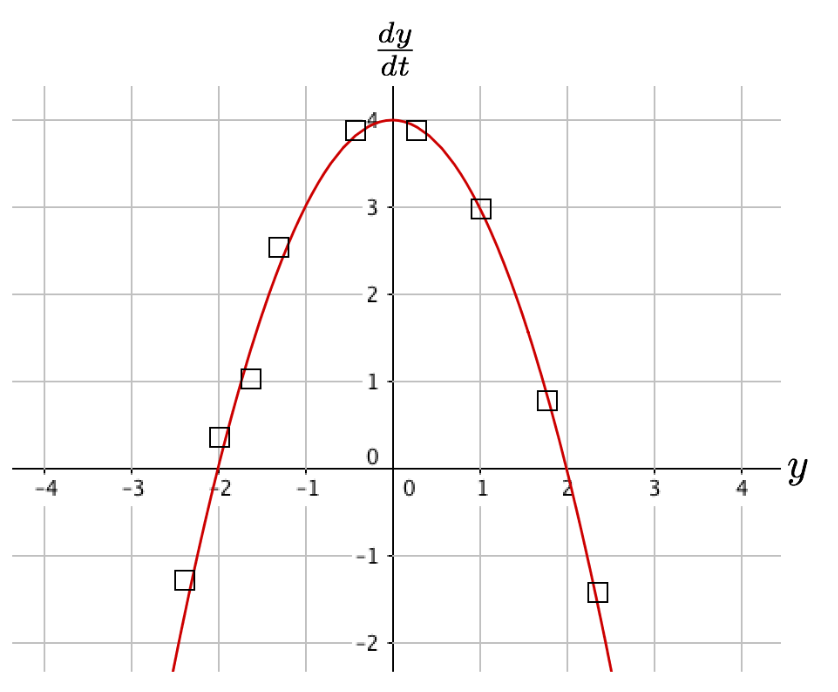
\includegraphics[width=3.5in]{07/07Bugs2.png}
\end{center}

\end{enumerate}

\clearpage
%%%%%%%%%%%%%%%%%%%%%%%%%%%%%%%%%%%%%%%%
\pagebegin{Homework Set 7}

\begin{enumerate}
\item  For this problem, use the coffee cooling rate of change equation  \[\displaystyle \frac{dC}{dt}=-0.4C+28.\] \label{07HWproblem1}
\begin{enumerate}
\item	Is there ever a time when two cups of coffee, one at initially 160\degree F and one at 180\degree F, are the exact same temperature? Answer this question according to the uniqueness theorem. Comment on whether your answer matches what you expect to happen in real life? 
\item	How long will it take a cup of hot coffee that is initially 180\degree F to cool down to 100\degree F? Use the reverse product rule to figure this out and then check the reasonableness of your answer with Euler's method.

\end{enumerate}
\item	For each part below you are provided with an autonomous derivative graph. Figure out the long-term behavior of every possible solution function. Illustrate your conclusions with representative $y(t)$ solution graphs and summarize your findings about the long-term behavior of different solutions in paragraph form. \label{07HWproblem2} \\
\begin{enumerate*}
\item 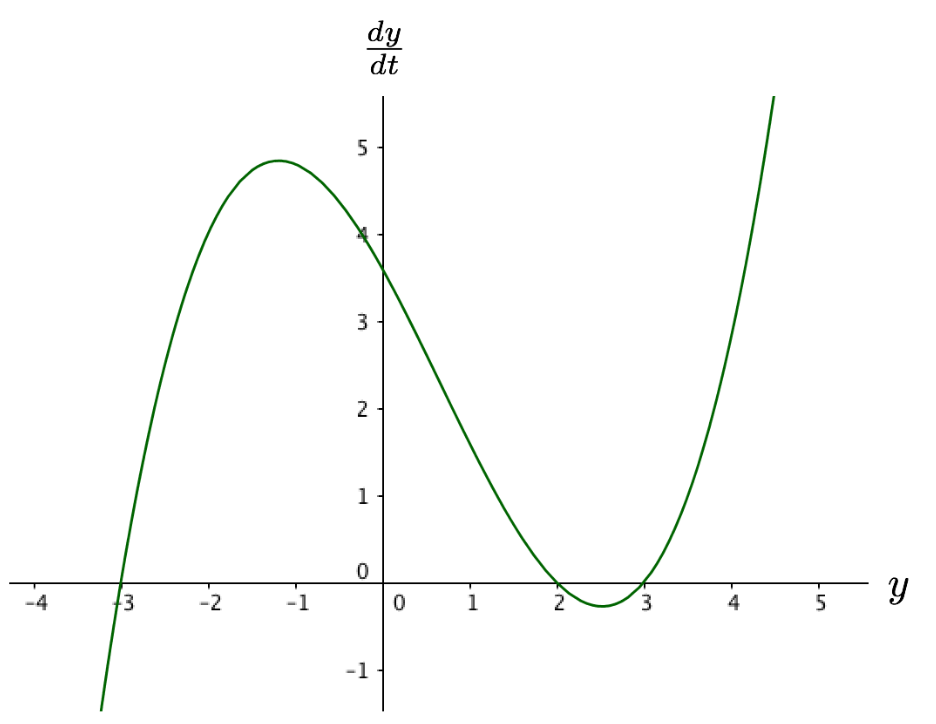
\includegraphics[width=3in]{07/07HWgraph1.png} \label{07HWproblem2parta}
\item 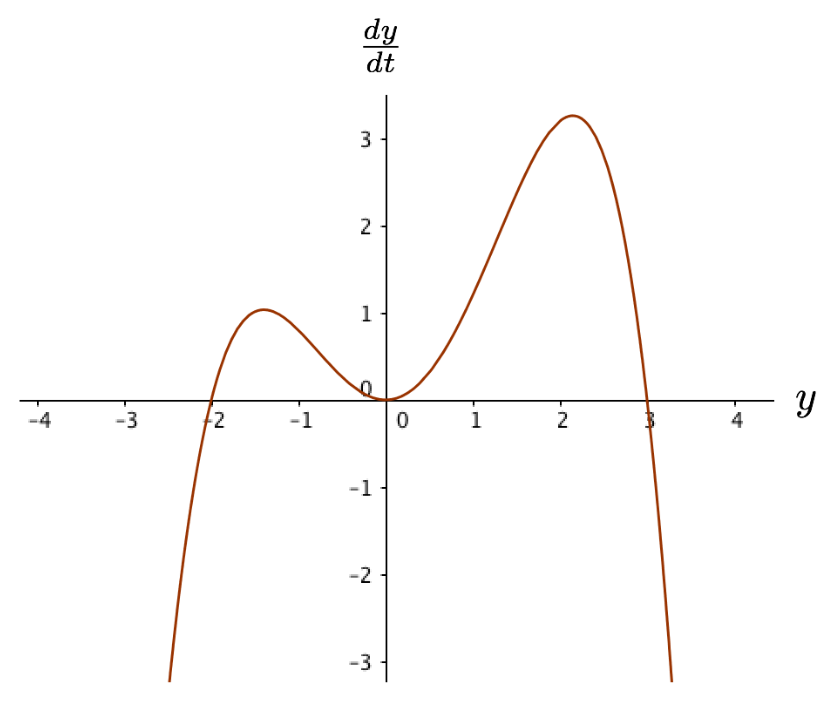
\includegraphics[width=3in]{07/07HWgraph2.png} \label{07HWproblem2partb}
\end{enumerate*}
\item	For each part in problem \ref{07HWproblem2}, create a phase line and classify each equilibrium solution as either an attractor, repeller, or node. \label{07HWproblem3}

\item	For problem \ref{07HWproblem2partb}, use the uniqueness theorem to determine if any of the non-constant solution functions ever reach the equilibrium solution of $y(t)=0$ in a finite amount of time. \label{07HWproblem4}

\item	Given an autonomous differential equation $\frac{dy}{dt}=f(y)$ , give a general strategy for how to use an autonomous derivative graph to determine the long term behavior of solution functions. \label{07HWproblem5}

\clearpage

\item	Suppose you wish to predict future values of some quantity, $y$, using an autonomous differential equation (that is, $dy/dt$ depends explicitly only on $y$). Experiments have been performed that give the following information: \label{07HWproblem6}
\begin{itemize}
\item	The only equilibrium solutions are $y(t)=0$, $y(t)=15$, and $y(t)=60$
\item	If the value of $y$ is 100, the quantity decreases
\item	If the value of $y$ is 30, the quantity increases
\item	If the value of $y$ is negative, the quantity increases
\end{itemize}

\begin{enumerate}
\item	How many different phase lines match the above? Sketch all possible phase lines. \label{07HWproblem6parta}
\item	Provide a rough sketch of an autonomous derivative graph for each of your phase lines in part \ref{07HWproblem6parta}. \label{07HWproblem6partb}
\item	For each of your different sketches in part \ref{07HWproblem6partb}, develop a differential equation that fits the basic features. \label{07HWproblem6partc}
\end{enumerate}
\item  In what ways is the letter $y$ in the differential equation $\frac{dy}{dt} = .3y$ both a variable and a function? In what ways is $\frac{dy}{dt}$ a function? \label{07HWproblem7}
\item Newton's law of cooling is an empirical law that states that an object immersed in a constant, ambient temperature will have its temperature change at a rate proportional to the difference between the its temperature and the ambient temperature. Explain how the cooling coffee problem reflects Newton's law of cooling. \label{07HWproblem8}
\item A body was found in a temperature controlled environment (i.e., you know the room temperature) and is subject to Newton's law of cooling. Explain why you only need the room temperature and the measurement of the body's temperature at two different times to give an estimate of the time of death. \label{07HWproblem9}
\item Are the following true or false statements? Explain your reasoning. \label{07HWproblem10}
\begin{enumerate}
\item If the autonomous derivative graph has a vertical tangent line at some point, then according to the uniqueness theorem, solutions to the differential equation are guaranteed to touch or cross at that point.  
\item If the autonomous derivative graph is a polynomial, then according to the uniqueness theorem, solutions to the differential equation are everywhere unique.
\end{enumerate}
\item \label{07HWproblem11}
\begin{enumerate}
\item Go to the glossary and identify all terms that are relevant to this unit and list those terms here.
\item Are there other vocabulary terms that you think are relevant for this unit that were not included? If yes, list them.
\end{enumerate}

\end{enumerate}



